\subsection{Case01 - Drop}
\label{xdp_wifi_case01}

En este caso de uso se probará que es posible descartar todos los paquetes recibidos haciendo uso de la tecnología XDP en un entorno inalámbrico. Para la realizar la prueba, primero se debe compilar el programa XDP y segundo levantar el escenario donde se va a realizar la prueba  de funcionamiento. En el proceso del levantamiento de la topología en Mininet-WiFi se anclará el binario a un interfaz del escenario, por lo que únicamente se tendrá que preocupar de observar los resultados cuando se genere tráfico que atraviese dicha interfaz.\\
\par
\vspace{0.5cm}
\textbf{Compilación}\\
\par

Para compilar el programa \gls{xdp} se ha dejado un Makefile preparado en este directorio al igual que en los casos de uso \gls{xdp} en entornos cableados. Por lo tanto, para compilarlo únicamente hay que seguir las indicaciones del bloque \ref{code:case01_xdp_wifi_compilacion}.

\begin{lstlisting}[language= bash, style=Consola, caption={Compilación programa XDP - Case01},label=code:case01_xdp_wifi_compilacion]
    # En caso de no haber entrado en el directorio asignado del caso de uso
    cd TFG/src/use_cases/xdp-wireless/case01
    
    
    # Hacemos uso del Makefile suministrado 
    sudo make
\end{lstlisting}
\vspace{0.5cm}

Si tiene dudas sobre el proceso de compilación del programa \gls{xdp} le recomendamos que vuelva al case02 (\gls{xdp} - Cableado \ref{xdp_ether_case02}) donde se hace referencia al \textit{flow} dispuesto para la compilación de los programas \gls{xdp}.



\vspace{1cm}
\textbf{Puesta en marcha del escenario}\\
\par

Para testear los programas \gls{xdp} en un entorno inalámbrico, se hará uso de Mininet-WiFi para emular las topologías de red. Para levantar el escenario solo se tendrá que ejecutar el script en Python que hace uso de la API de Mininet-WiFi para generar toda la topología de red. Una vez ejecutado este abrirá la interfaz de linea de comandos de Mininet-WiFi, desde la cual se podrá comprobar el funcionamiento del caso de uso. En este caso, se realiza la carga del programa \gls{xdp} desde el propio script de Python, haciendo uso de la herramienta xdp\_loader desarrollada para ello. Por tanto, como se ha dicho este script está auto-contenido, por lo que solo se deberá ejecutarlo. \\
\par

Para limpiar la máquina del escenario recreado anteriormente con Mininet-WiFi se podría realizar un \texttt{sudo mn -c}, pero se recomienda al usuario que haga uso del \textit{target} del Makefile destinado para ello, ya que adicionalmente limpiará los ficheros intermedios generados en el proceso de compilación de nuestro programa \gls{xdp}. Ejecutando el siguiente comando se limpiaría la máquina.

\begin{lstlisting}[language= bash, style=Consola, caption={Compilación programa XDP - Case01},label=code:case01_xdp_wifi_run]
    # Levantamos el escenario
    sudo python runenv.py
    
    
    # Limpiamos el escenario
    sudo make clean
\end{lstlisting}
\vspace{0.5cm}

Por último, únicamente indicar que el escenario recreado es el siguiente, compuesto exclusivamente de dos estaciones \textit{wireless}, aisladas en sus propias \textit{Network Namespaces}, y un punto de acceso corriendo el \textit{daemon} de HostApd para intercomunicar dichas estaciones WiFi.

% figura escenario
\begin{figure}[ht]
    \centering
    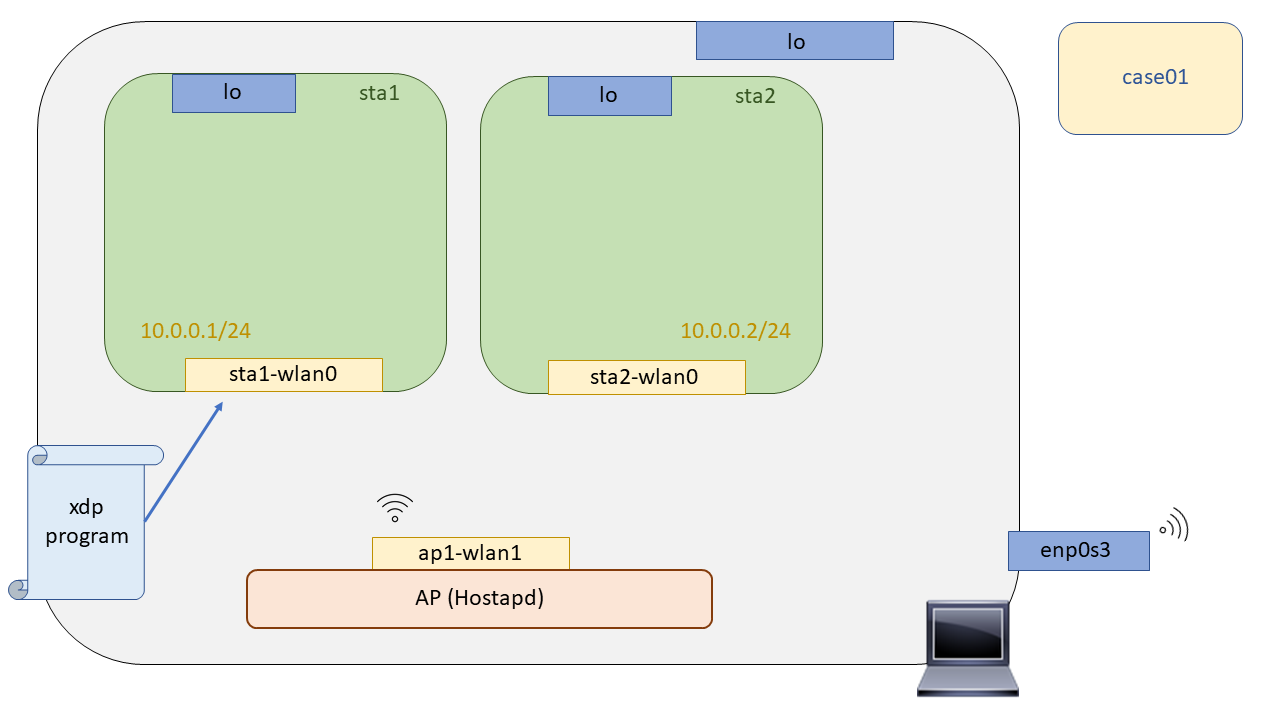
\includegraphics[width=16cm]{archivos/img/dev/xdp-wifi/case01/scenario.png}
    \caption{Escenario inalámbrico del Case01 - XDP}
    \label{fig:case01_xdp_wifi_scenario}
\end{figure}

\vspace{0.5cm}
\textbf{Carga del programa XDP}\\
\par

Como ya se ha comentado, la carga del programa \gls{xdp}, se llevará a cabo en el proceso del levantamiento del escenario, descrito en el script de Python para crear la topología. La carga del programa \gls{xdp}, se hará con el programa \texttt{xdp\_loader}, utilizado anteriormente para cargar los programas \gls{xdp} en interfaces alámbricas. 

\begin{lstlisting}[language= bash, style=Consola, caption={Carga del programa XDP - Case01},label=code:case01_xdp_wifi_load]
    # Linea 38 del script runenv.py
    sta1.cmd("./xdp_loader -S -d sta1-wlan0 -F --progsec xdp_case01")
\end{lstlisting}
\newpage
Es importante señalar, que el comando ejecutado dentro de la \textit{Network Namespace} de la estación WiFi \texttt{sta1}, no se ha lanzado con permisos de root, ya que esta orden los heredará al lanzar el script que levanta la topología en Mininet-WiFi. 

\vspace{1cm}
\textbf{Comprobación del funcionamiento}\\
\par

Una vez que el programa \gls{xdp} fue anclado a la interfaz de la estación WiFi \texttt{sta1}, es necesario comprobar si realmente funciona según lo esperado, y ver si las interfaces generadas por el módulo mac80211\_hwsim son compatibles con \gls{xdp}. Esto se hará generando tráfico desde una estación WiFi hacia la otra, para que atraviese por la interfaz que tiene anclado el programa \gls{xdp}. En este caso el comportamiento esperado es que haga un \textit{drop} de los paquetes nada más llegar a la interfaz, en este caso la interfaz \texttt{sta1-wlan0}.\\
\par
Como en anteriores casos de uso, se ha habilitado la recolección de estadísticas sobre los códigos de retorno \gls{xdp}, por lo que sería una buena práctica comprobar si se están empleando códigos de retorno \texttt{XDP\_DROP}.


% figura escenario
\begin{figure}[ht]
    \centering
    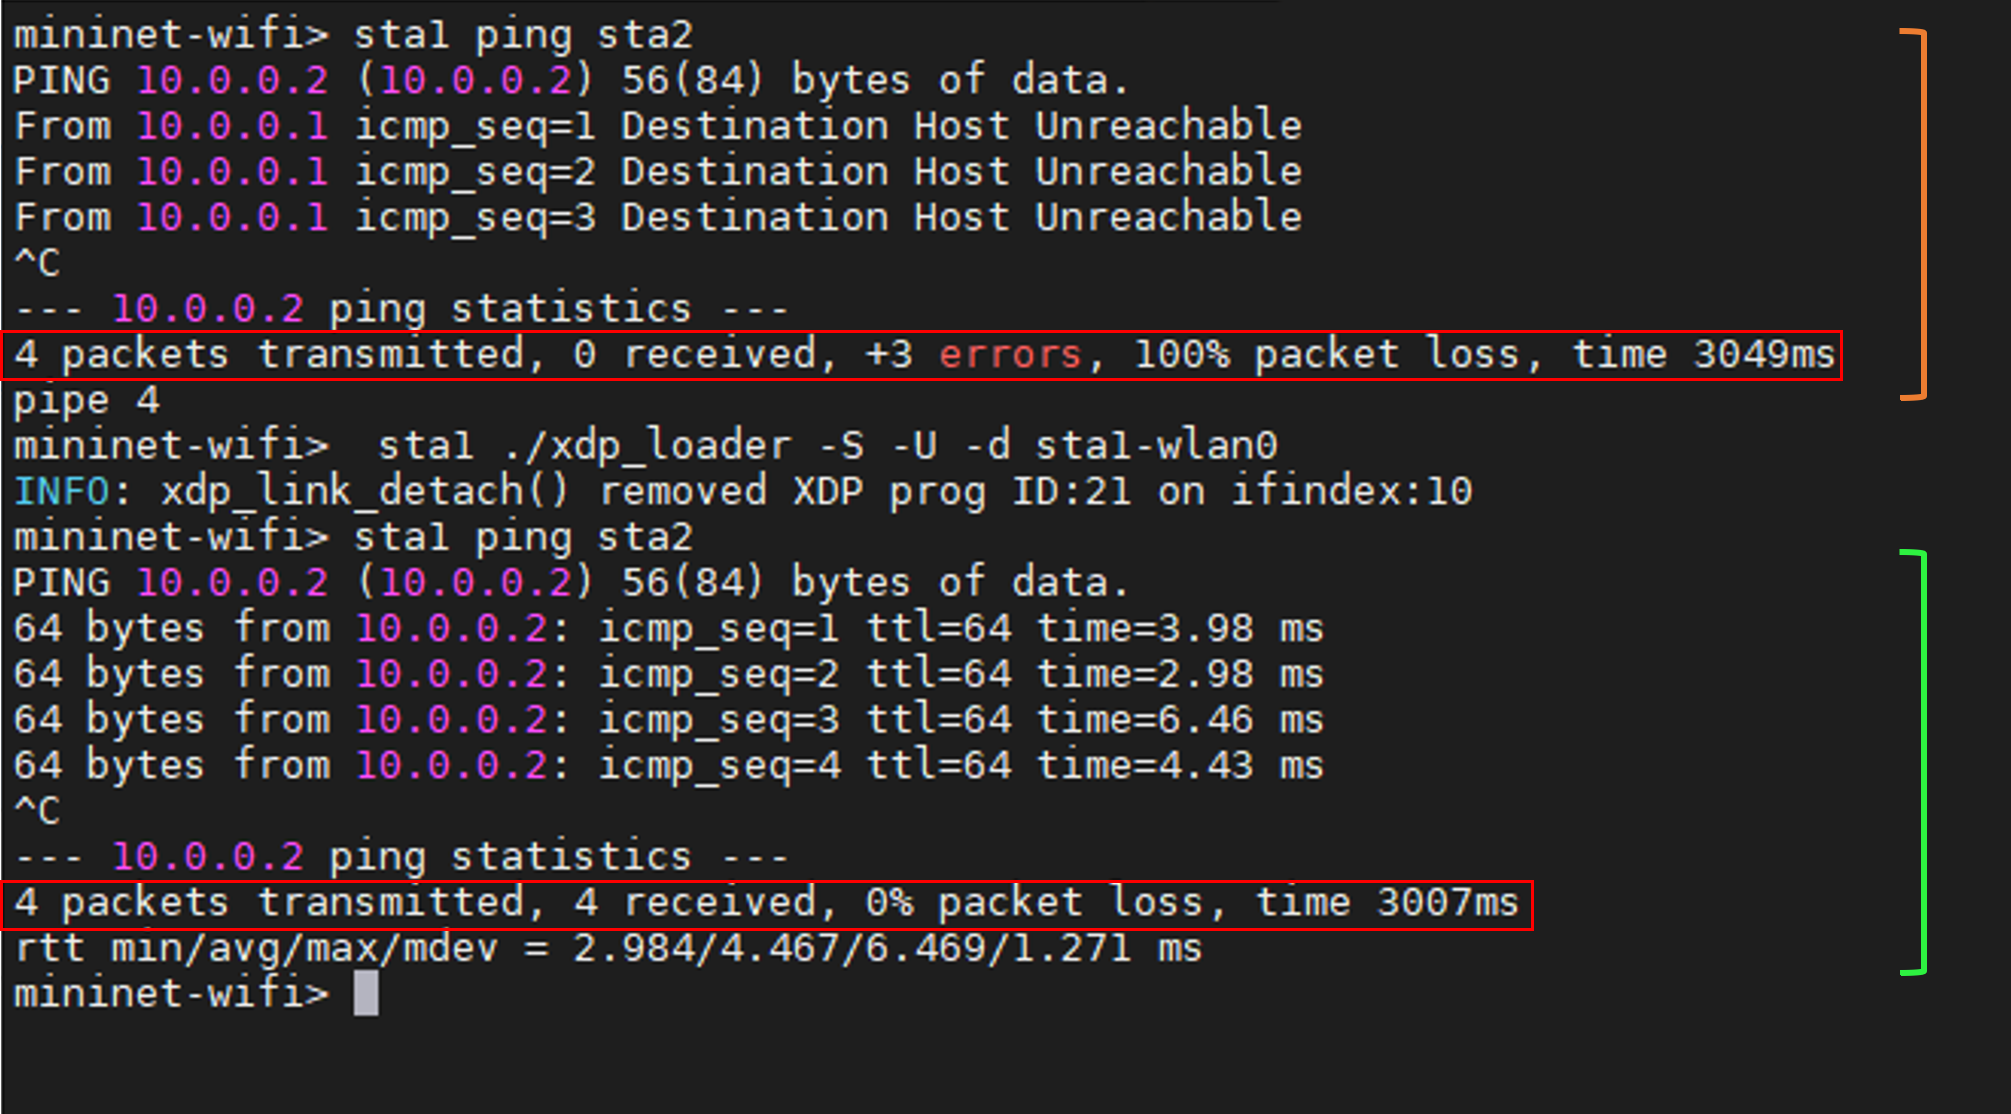
\includegraphics[width=14cm]{archivos/img/dev/xdp-wifi/case01/demo_case01_edited.png}
    \caption{Comprobación de funcionamiento del Case01 - XDP Wireless}
    \label{fig:case01_xdp_wifi_func}
\end{figure}

Como se puede apreciar en la figura \ref{fig:case01_xdp_wifi_func}, inicialmente se realiza un ping \fcolorbox{black}{orange}{\rule{0pt}{2.5pt}\rule{2.5pt}{0pt}}\hspace{1mm} entre las estaciones WiFi, pero no hay conectividad debido a que el programa \gls{xdp} está tirando los paquetes. Acto seguido se quita el programa \gls{xdp} de la interfaz y se vuelve a probar la conectividad entre las estaciones WiFi ejecutando un segundo ping \fcolorbox{black}{green}{\rule{0pt}{2.5pt}\rule{2.5pt}{0pt}}\hspace{1mm}. Se ve que una vez desanclado el programa, la conectividad vuelve, por lo que se puede afirmar que el funcionamiento es el esperado.  